% !TEX root = main.tex
\section{Method}

\subsection{Programming a BWIM system}
Describe shortly how the BWIM system have been programmed.
Keywords:
\begin{itemize}
\item Beam bridge model
\item Producing a strain history through influence lines
\item Finding the speed of the train
\item Finding Axle distances
\item Solving system for axle weights
\end{itemize}
This master project began by learning how a BWIM-system works, and to then create a working model performing BWIM. To not make this a too big project this meant building a simple beam model of a bridge in Matlab, and simulate moving loads crossing it.

A simple flow diagram describing the intial BWIM program:
\begin{figure}
% 
\tikzset{
  terminal/.style={draw, rounded rectangle, text width=3cm, text centered},
  process/.style={draw, text width=3cm, text centered},
  decision/.style={draw, diamond, aspect=2, text width=3cm, text centered},
  delay/.style={draw, rounded rectangle, rounded rectangle west arc=none, text width=3cm, minimum height=1cm, text centered},
  line/.style={draw, -latex}
}
\begin{tikzpicture}
  \node[terminal] (main) {Main script};
  \node[process, above=1cm of main] (createInfl) {create influence line};
  \node[process, right=2cm of main] (createStrain) {create strain signal};
  \node[process, below=2cm of main] (findSpeed) {find train speed};
  \node[process, left=1cm of findSpeed] (findAxleDist) {find axle distances};
  \node[process, left=2cm of main] (calcAxleWeights) {calculate axle weights};

  \draw[line] (main) -- (createInfl);
  \draw[line] (main) -- (createStrain);
  \draw[line] (main) -- (findSpeed);
  \draw[line] (findSpeed.west) -- (findAxleDist.east);
  \draw[line] (main) -- (calcAxleWeights);
\end{tikzpicture}%

\end{figure}


\subsubsection{Producing a strain signal}
Through the theoretical moment influence lines of the beam, a strain signal can be built through the moment-strain relationship, found in equation\ref{equation:moment_strain}, for a given set of axle weights. A simple beam bridge model, as seen in figure \ref{figure:beam_model}, will not recreate a actual bridge strain signal but will be used to create a working BWIM system. The produced strain signal will differ from an actual strain signal mostly because of dynamics, from the train and bridge, and because actual boundary conditions of a bridge will differ from the boundary conditions of a simple beam model. The strain sensors will also produce noise distorting the signal.

To make as good a signal as possible, some effort were placed into recreating the effect mentioned above. To add noise to the signal, white gaussian noise was included in the signal through Matlabs wgn function "http://se.mathworks.com/help/comm/ref/wgn.html".


This strain signal could then be used as a base to build the code for a BWIM system.

\begin{figure}
	\begin{tikzpicture}
		\draw[thick] (0,0) to (5,0);
		\node[ledd fast={0}{0}{0}] (ledd) {};
		\node[ledd skyve={5}{0}{0}] (skyveledd) {};
		%\draw[->] (0,1) to {$\scriptstyle g$} (0,.1);
		\node (a) at (1,1.5) {};
		\node (b) at (1,.1) {};
		\draw[-open triangle 90] (a) to node[pos=-.4] {$axle 2$} (b);
		\node (c) at (3.5,1.5) {};
		\node (d) at (3.5,.1) {};
		\draw[-open triangle 90] (c) to node[pos=-.4] {$axle 1$} (d);
		\node (e) at (3.5,1) {};
		\node (f) at (4.5,1) {};
		\draw[-open triangle 90] (e) to node[pos=1.2] {$v$} (f);
		\node (g) at (1,.5) {};
		\node (h) at (3.5,.5) {};
		\draw[open triangle 90-open triangle 90] (g) to node[above] {$axle spacing$} (h);
		%\draw (2.5,0) circle [radius=0.1] {sensor};
		%\node[draw,circle] (s) at (2.5,0){};
		\filldraw
		(2.5,0) circle (2pt) node[align=left,   below] {strain sensor};
	\end{tikzpicture}
%\captionof{figure}{Beam model for initial BWIM}
\caption{Beam model for developement}
\label{figure:beam_model}

\end{figure}


\subsubsection{Finding the speed of the train}
Two working methods of finding the speed of a passing train were developed:
\begin{itemize}
 \item By identifying peaks in the strain history for two different sensors, representing the same axle. The distance between the two sensors and the time difference between the found peaks should theoretically give a good estimate of the trains velocity.
 \item Through doing cross correlation between two sensors strain history. This involves finding the phase difference, or lag, between the signals. The known distance between the strain gauges should then along with a constant, based on distance between sensors, give a reliable estimate of train velocity. INSERT PLOT OF CORRELATION AND SHOW MATHEMATICAL EQUATION DESCRIBING CROSS CORRELATION.
\end{itemize}

\subsection{Finding influence lines}
Describe how influence lines have been found from the given strain history from Lerelva Bridge.
Keywords:
\begin{itemize}
\item Matrix method
\item Optimization
\item Speed
\end{itemize}
\subsubsection{Matrix method}
Describe the matrix method.

\subsubsection{Optimization}
Describe how optimization can be used to find optimal influence lines for the bridge.

\subsection{System setup}
\label{system_setup}
To test the BWIM-program on actual data, we Gunnstein, Daniel set up a BWIM-system to gather strain data from actual train passings. The subject bridge were Lerelva-Bridge in Trondheim, figure \ref{fig:lerelva_bridge}, a typical Norwegian steel railway bridge. Three strain gauges, \SI{3}{\mm} \SI{120}{ohms} from HBM, were placed by the support towards Trondheim on the first section of the longitudinal stringer, see figure \ref{fig:strain_gauges}. The sensors were placed with \SI{1}{\m} spacing around the middle of the stringer section. These strain gauges were connected to a National Instruments compactDAQ with module NI 9235 which produced an continuous data flow to a standard laptop, see figure \ref{fig:instruments}. A Kipor generator was brought for power.
% INSERT SYSTEM IMAGE HERE
\begin{figure}[H]
	\centering
	\begin{subfigure}[t]{0.49\textwidth}
    \centering
    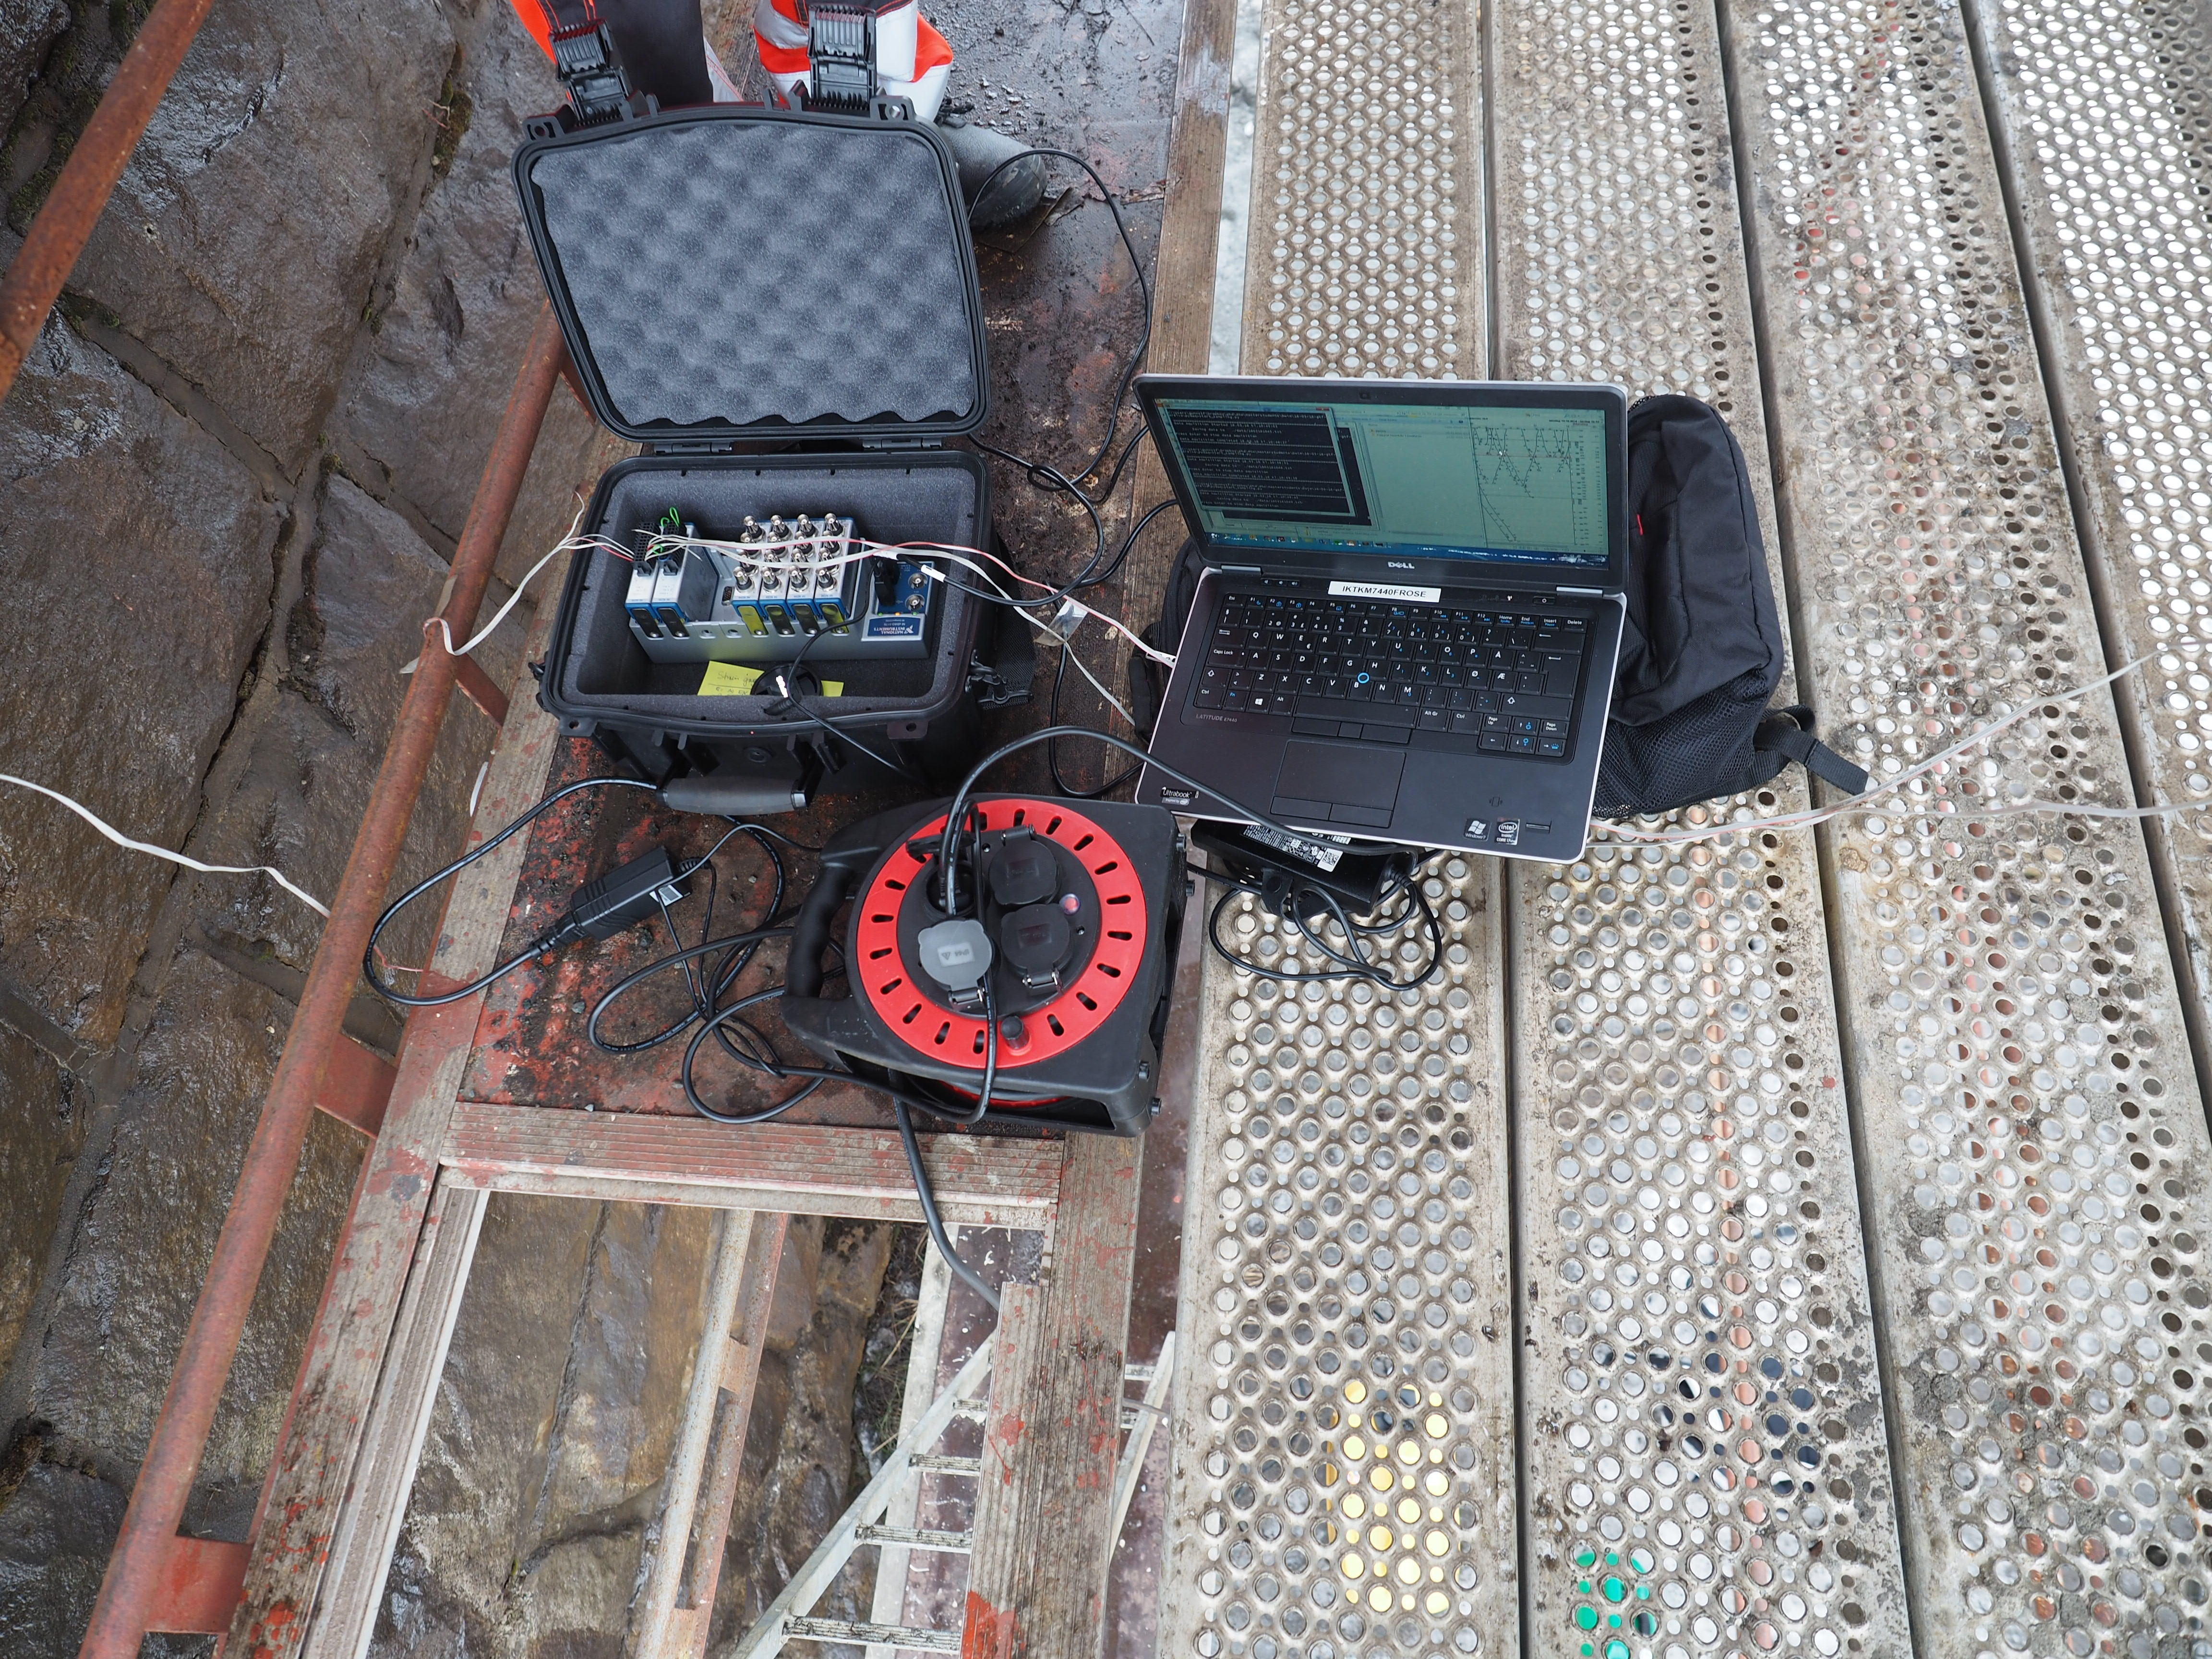
\includegraphics[width=\textwidth]{figures/2016-03-16/system_setup}
		\caption{System setup from data gathering at Lerelva}
		\label{fig:instruments}
	\end{subfigure}
	\begin{subfigure}[t]{0.49\textwidth}
    \centering
    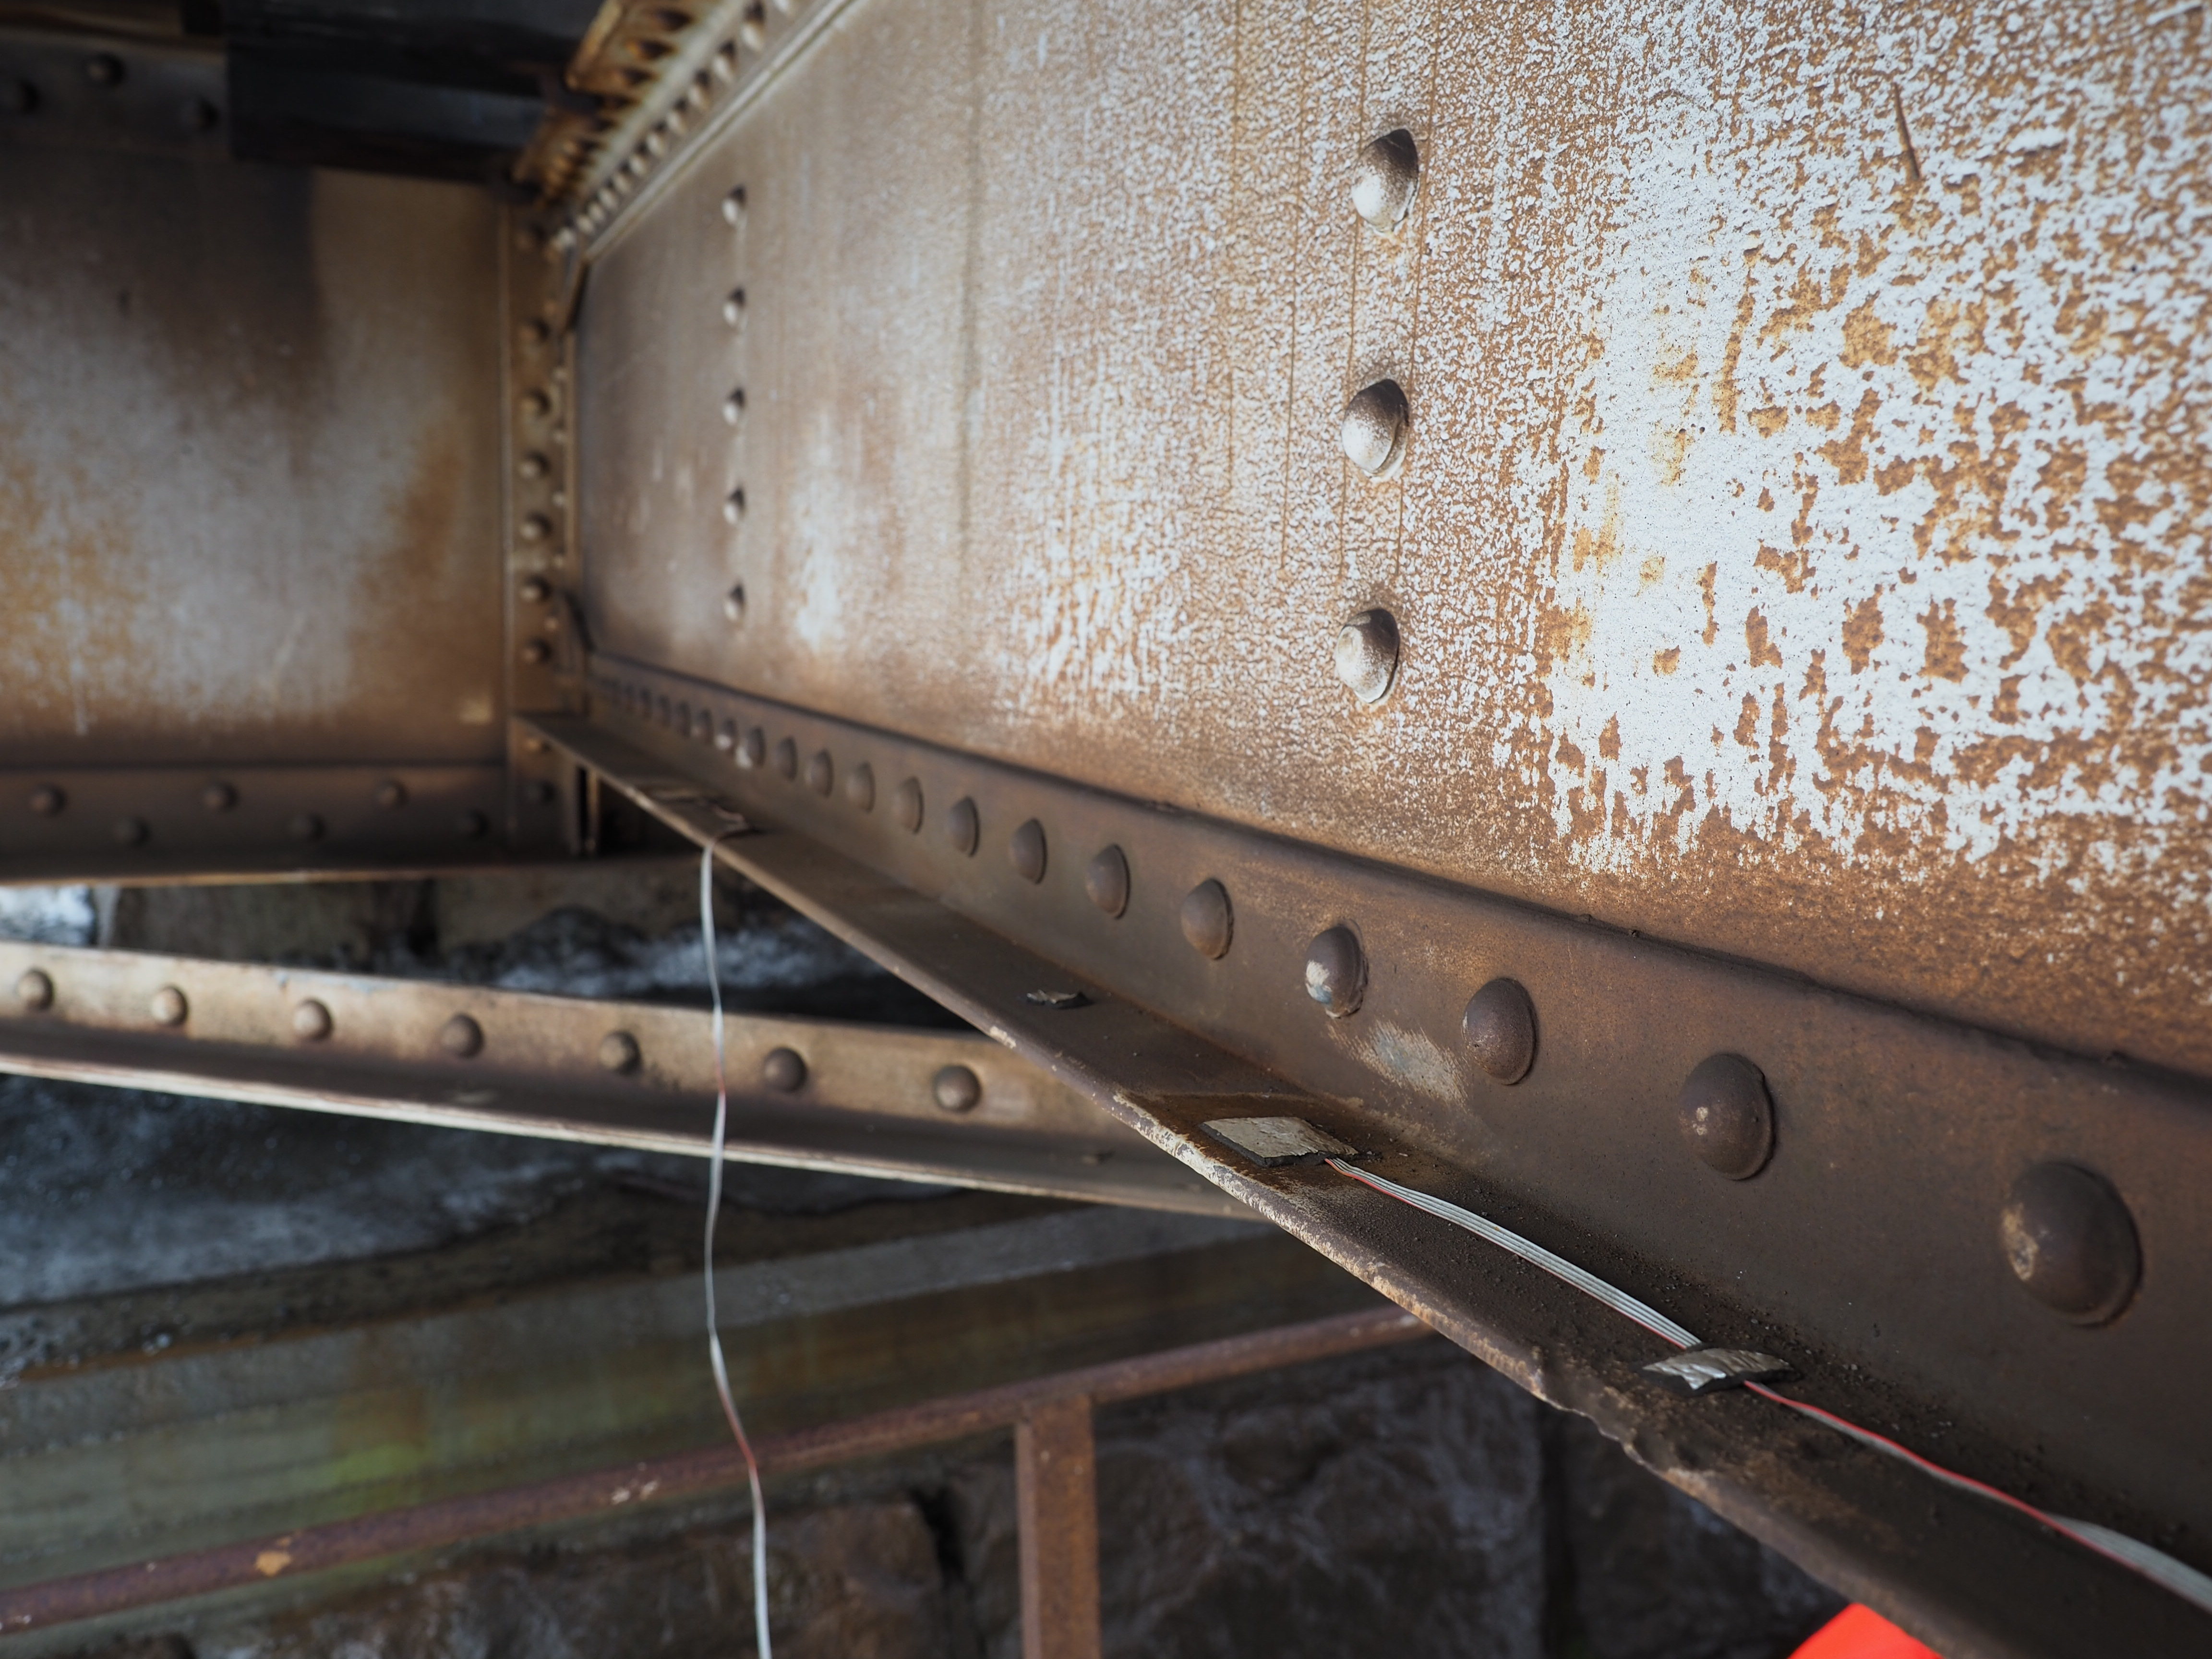
\includegraphics[width=\textwidth]{figures/2016-03-16/sensor_placement}
		\caption{Placement of strain gauges on stringer section}
		\label{fig:strain_gauges}
	\end{subfigure}
	\caption{Instruments for aquiring strain data}
	\label{fig:system_setup}
	% 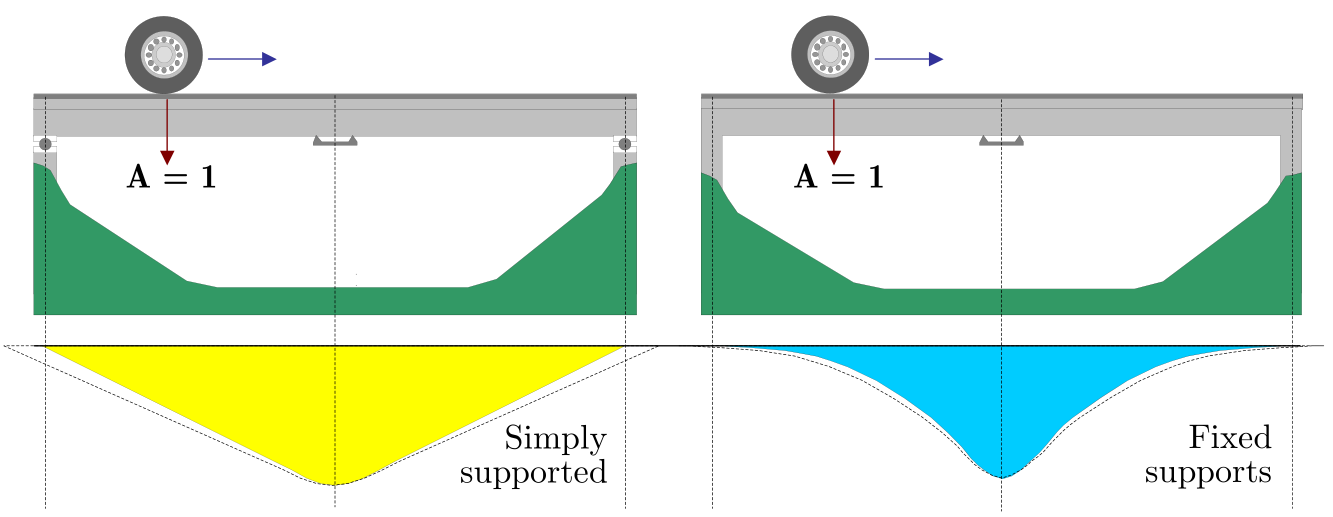
\includegraphics[scale=0.5]{figures/inflLinesQuilligan}
\end{figure}
\begin{figure}[H]
	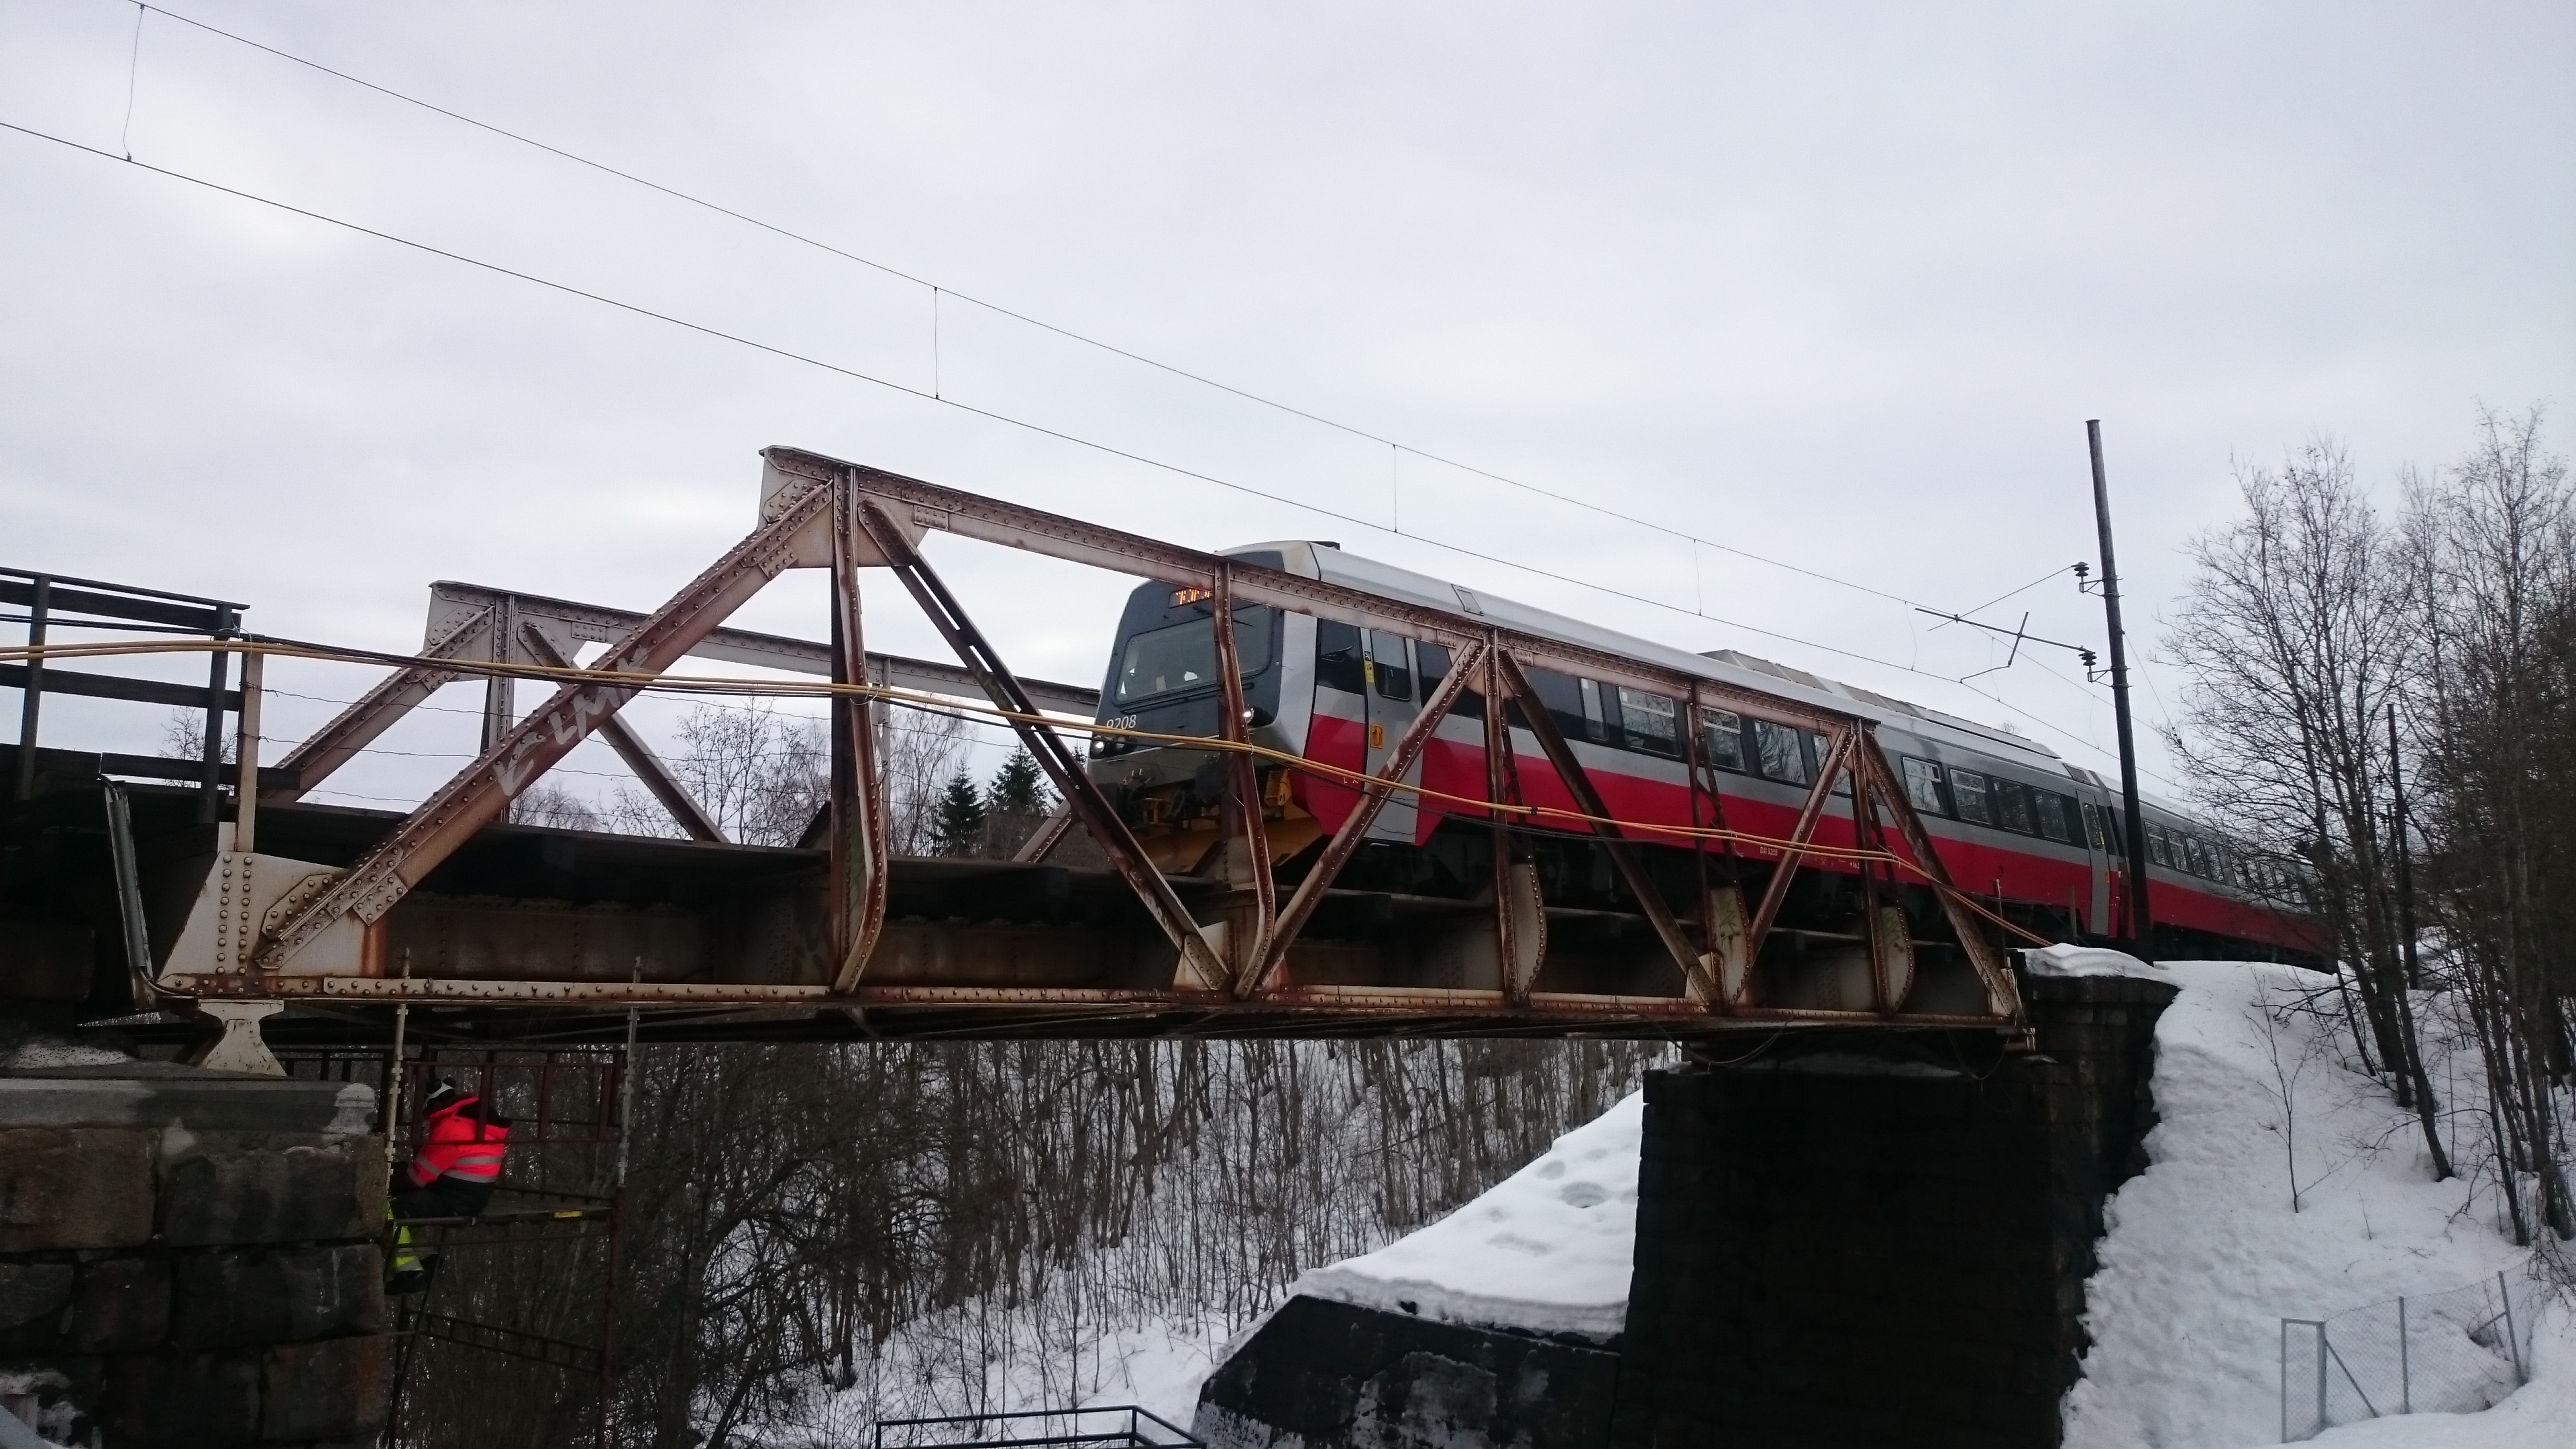
\includegraphics[width=\textwidth]{figures/2016-03-16/train_passing.jpg}
	\caption{Lerelva bridge with a train passing over}
	\label{fig:lerelva_bridge}
\end{figure}


\subsection{Testing}
Keywords:
\begin{itemize}
\item Comparing calculated strain with measured strain
\end{itemize}
